% https://books.google.com/books?id=QQJODwAAQBAJ&pg=PA101&lpg=PA101&dq=%E2%80%9Cthe+secret+to+successful+hiring+is+this:+look+for+the+people+who+want+to+change+the+world.%E2%80%9D&source=bl&ots=D6l8JXfB20&sig=ACfU3U0x1X9Gh8k6MlNV0BqhBa_73Q0yfQ&hl=en&sa=X&ved=2ahUKEwj48pqg_oHgAhVohuAKHYlJAsc4ChDoATAAegQIChAB#v=onepage&q=%E2%80%9Cthe%20secret%20to%20successful%20hiring%20is%20this%3A%20look%20for%20the%20people%20who%20want%20to%20change%20the%20world.%E2%80%9D&f=false
% "The secret to successful hiring is this: look for the people who want to change the world.".  Marc Benioff.

NumPy is both a cause and an effect of a striking shift in the nature of
scientific computing.  In the traditional scientific software model, the user is a {\it consumer}.  Writing software is a task for specialists and
professionals, supported by income from selling the software to
scientists.  In the new model, the user is an {\it owner}.  The Python language, with
the NumPy library, provides a framework that scientists can consume,
but also encourages scientists to participate as programmers---to
write code for the library and the ecosystem of packages around it.  This has
fostered a new culture of contribution and collaboration in scientific
computing that resulted in a virtuous cycle of increasing use, and increasing
development.

This cycle is one of several explanations for the astonishing growth of NumPy
in scientific computing.

\section*{History}

The first incarnation of NumPy was a package called Numeric, written in 1995
by Jim Hugunin, then completing his master's thesis at MIT on
superconductor-semiconductor junctions.  Hugunin based his package on previous
work by Jim Fulton, then working at the US Geological Survey, and acknowledges
many others in his initial report of the package \cite{Hugunin-whitepaper}.
Numeric provided an array object in Python, written in C, and linking to
standard fast implementations of linear algebra.
% https://stackoverflow.com/questions/26948776/where-did-the-term-broadcasting-come-from/26950256
% https://mail.python.org/pipermail/matrix-sig/1995-November/000143.html
% May want to mention Yorick here (origin of broadcasting idea)

As Hugunin points out, at the time he wrote Numeric, commercial languages for
interactive computing with numerical arrays were already well-established,
including Matlab and IDL.  Back then, it must have seemed a safe bet that
Numeric would not succeed in this market.  The commercial languages were
developed and maintained by large groups of full-time professional programmers,
supported by formal quality assurance, release managers, and writers of
scientific documentation.  In contrast, Numeric, and later NumPy, would
continue to be developed almost entirely by scientists, including graduate
students and faculty, without specific funding and often to the detriment of their careers.
% S: The "Back then" sentence sets up an expectation.  Later in this section, we then explain that Numeric/NumPy *was* successful, but we never explicitly close the loop: "despite the odds, great success".

%Table X1 about here: backgrounds of initial designers (mainly math, physics).

%Table X2 about here: backgrounds of major committers (mainly math, physics).

% S TODO: the first sentence below could flow a bit better
Around 1998, the Space Telescope Science Institute (STScI) software group began
to use Python heavily and, around 2000, wrote a re-implementation of much of
Numeric, called NumArray, to support their need to work on large memory-mapped
arrays and arrays of mixed data type records \cite{STScI-slither}.  This
briefly caused the Numeric and NumArray communities to diverge, until 2005,
when Travis Oliphant embarked upon a major rewrite that aimed to be a ``best of
both worlds'' unification of Numeric and NumArray \cite{oliphant2006guide}.
This merger resulted in NumPy.  At the time, Oliphant was an assistant
professor of Electrical and Computer Engineering at Brigham Young University.

Over the next 10 years, NumPy attracted a relatively large pool of scientist
developers.  To benefit from these
user-developers, the project developed an increasingly strong culture of using
software-engineering practice to improve collaboration and reduce error
\cite{millman2014developing}. The NumPy team was early in adopting distributed
revision control and code review to improve collaboration on code, and
continuous testing that runs a large battery of automated tests for every proposed
change to NumPy. At first, NumPy had rather sparse documentation, but the project
developed a new standard for ``docstrings''---text describing each NumPy
function---and used this standard to write comprehensive, high-quality
documentation, integrated with the source code\cite{vanderwalt2008scipy,harrington2008scipy,harrington2009scipy}. The NumPy documentation format
quickly became a standard for the larger Python community.

NumPy now underpins almost every Python library that does scientific or
numerical computation, including SciPy\cite{virtanen2019scipy},
matplotlib\cite{hunter2007matplotlib}, pandas\cite{mckinney-proc-scipy-2010},
scikit-learn\cite{pedregosa2011scikit}, and
scikit-image\cite{vanderwalt2014scikit}.
NumPy consists of the $n$-dimensional array object along with utility functions
that operate on it.
Because of its inherent simplicity---being a pointer to memory with some
associated meta-data about shape, data-type, and so forth---the NumPy array is
the {\it de facto} exchange format for array data in Python.
The library has such widespread adoption that not only the array object but also its
{\it Application Programming Interface} (API) has become ubiquitous as
a language for tensor computation---witnessed by its use in popular
deep learning libraries such as PyTorch\cite{pytorch}.

\section*{Enabling factors}

The creation of NumPy spurred renewed development in the larger scientific
Python ecosystem and heralded the current era of wide-spread use of Python for
scientific computing.
As we implied above, there were several factors that allowed this rapid growth
and successful development.

Hugunin identified the first factor in his initial description of the Numeric
package \cite{Hugunin-whitepaper}.  Numerical computing is usually one
component of a larger programming task, therefore:

\begin{quote}
    Rather than trying to retrofit an existing numerical language to support
    the wealth of features found in a powerful, modern, general-purpose
    programming language, it makes much more sense to attack the problem from
    the other direction and add the features of a powerful numerical
    programming language to Python.
\end{quote}

Python is already a good choice for many standard programming tasks such as
cleaning data, interacting with web resources and parsing text.  It has a wide
range of libraries for many different tasks. Adding fast array operations and
linear algebra allows the scientist to do all their work with within the same
language---and one that has the advantage of being famously easy to learn and
teach.

The second factor flows from Python's nature as an open-source language,
embedded within the open-source community.  Python attracts developers who like
to build and contribute.  As a result, NumPy has always been a library that was
developed by scientists in order to do their work.  Commercial specialist
numerical languages can encourage consumer-users, who pick up a tool and use
it, but do not expect to contribute to development%<-sentence a bit tough to parse.
In contrast, NumPy often
attracts user-developers, who want to work with NumPy, and are prepared to fix
and extend the library as they work. User-developers have been the fundamental
force in developing NumPy, and shaping it into a library that has been refined
in the furnace of practical scientific work.

The third factor is much like the second: a culture in Python that concentrates
on high quality of code and distribution. Because Python is open-source, it has
a strong culture of contribution, and therefore, of using tools and process to
improve collaborative software development, such as distributed version
control, code review, and automated testing.  These have allowed the project to
scale safely as it attracted more users and developers, even though these
developers rarely came to the project with training in software engineering.

Lastly, we believe NumPy has benefited greatly from a well-chosen application
programming interface (API).  Scientific and numerical programming needs to be
fast, and scale to very large datasets.  The NumPy API defines a simple wrapper
for data in memory so it can be represented as a one- or multi-dimensional
array.  The simplicity of this wrapper has made it very successful as a
standard way of representing arrays in memory, and has made it relatively easy
for other libraries to develop fast and memory-efficient compiled code, usually
in C or Fortran, that can manipulate these arrays and pass them back to Python.
This has been a large factor in the growth of numerical computing libraries
around NumPy and Python.

% S: I think two issues are conflated here: the simple underlying memory model, and the API.  The API has developed organically, while the underlying memory model is a design decision that shapes much of how the rest of the library was built.

% S:
%
% Thinking about enabling factors, I'd characterize them into three categories:
%
% - Practical
% - Philosophical
% - Social
%
% E.g., practical: reason why we use Python (learn one language for everything); students don't have money, so want to avoid impracticalities of license dongles/servers, etc.
%
% Philosophical: science should be open, transparent; our software should be controlled by scientists, not designers that we don't have access to
%
% Social: joy of building these things together, friendly welcome into the community for many of us---appreciation of our work and hours
%

\section*{NumPy arrays}

The NumPy array data structure stores regularly spaced elements of a single
data type in a contiguous block of memory; along with meta-data such as shape,
it allows for the efficient representation of $n$-dimensional arrays \cite{vanderwalt2011numpy}.
The need for such a data structure arises often in science.
For instance, they may store measurements from an experiment or simulation
at discrete time points.

Data analysis frequently involves operations $(+, -, \times, /, \log, \sin, \dots)$ on
the individual measurements.
In programming languages such as C or Java, this would involve looping over
every element to perform these operations.
Array computations generalize these element-wise operations on scalars to
vectors (1-d arrays), matrices (2-d arrays), and higher dimensional arrays (n-d
arrays).
For instance, if \code{x} is an array, then \code{2 * x} produces
an array whose values are twice those in \code{x}.
Similarly, if \code{x} and \code{y} have the same shape, then
\code{x * y} produces an array whose values are the products of
the corresponding entries of \code{x} and \code{y}.
When \code{x} and \code{y} have different shapes, the smaller array is \emph{broadcast}
across the larger array to a common shape when sensible.
For example, if \code{x} is a 1-d array with length 3, and \code{y} is a 2-d
array with shape $2 \times 1$, the output will be an array with shape $2 \times 3$
(see Figure~\ref{fig:broadcasting}).

\begin{figure}
  \centering
  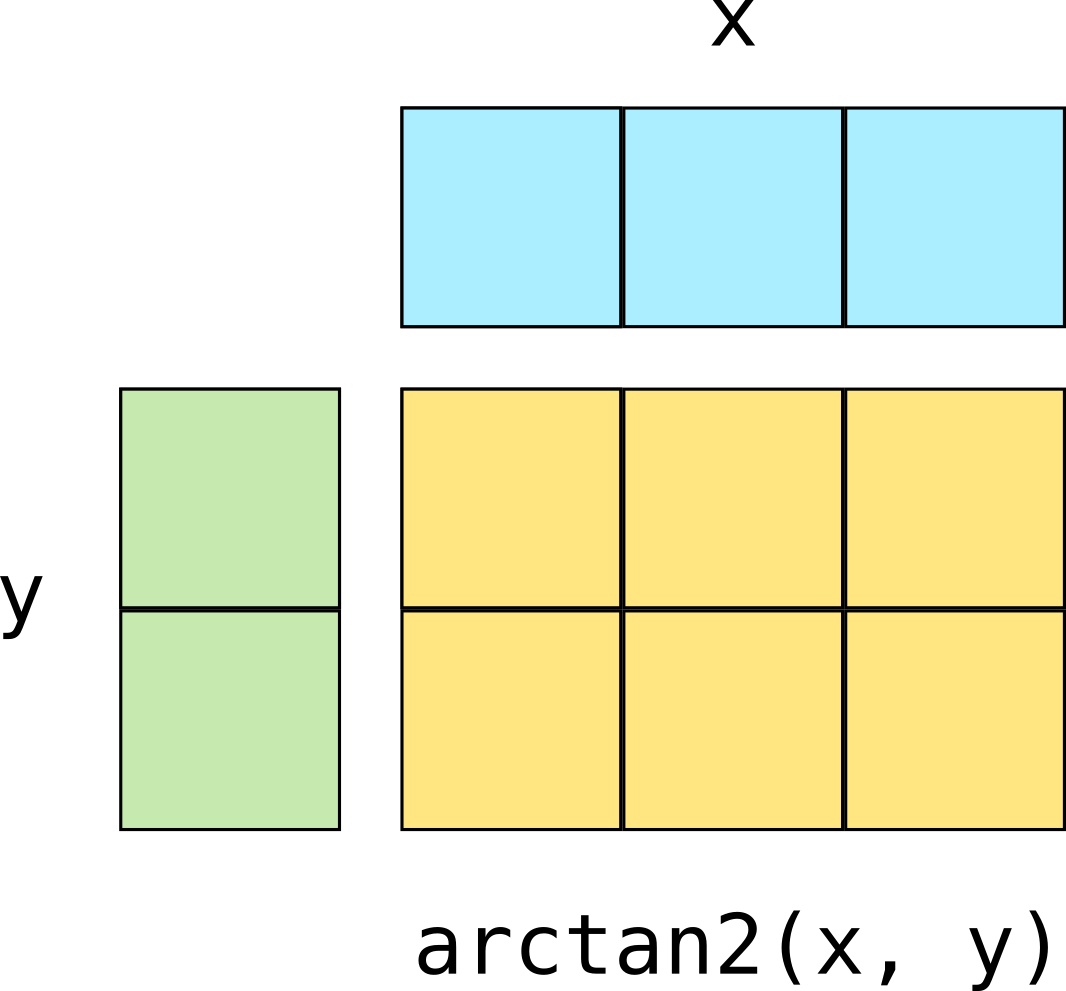
\includegraphics[width=0.5\linewidth]{static/broadcasting}
  \caption{
    Broadcasting a $1 \times 3$ array against a $2 \times 1$ array
    yields a $2 \times 3$ result.
  }
  \label{fig:broadcasting}
\end{figure}

These vectorized operations often produce one-liners that would be many tens
of lines of code in languages such as C.

Element-wise operations are not always desired.
Suppose the matrix \code{A} is a 2-d array and the vector \code{x} is 1-d array.
Then \code{A @ x} computes the matrix-vector product $Ax$ and
\code{x @ A} computes the vector-matrix product $x^\top A$.
This matrix multiplication operation extends to higher-dimensions by
treating the array as a stack of matrices.

NumPy also provides a large collection of functions for array manipulation
including functions for:
creating, reshaping, concatenating, and padding arrays;
searching, sorting and counting data in arrays;
computing elementary statistics, such as the mean, median, variance, and standard deviation;
reading and writing files;
and more.
It also provides extensive support for generating pseudorandom numbers
as well as an assortment of probability distributions.
For historical reasons, NumPy also includes basic functionality for
linear algebra, fast Fourier transforms and windowing,
and polynomial fitting.
We will continue supporting these, but we will not expand beyond them.

\section*{Recent development}

For many years, NumPy had no dedicated funding, and development time
was mostly contributed freely by students and researchers in their
spare time.  In-person meetings were sponsored off of individual's
research grants, and while industry sponsored contributions were made,
notably those by Mark Wiebe when he was sponsored by Travis Oliphant
at Enthought, the package's rapid adoption in scientific
computing took place without external investment.

In 2018, we hired our first full-time developers.

- advantages of full-time developers

- concerns about adding paid, full-time developers to our culture of user-developer volunteers

- how we avoided these concerns

1. hired mostly community members
2. carefully planned work with community input
3. focus on helping community (code review)


The first activities organized for the new grants were a development planning
sprint, a weekly community call, and a meeting to write a draft roadmap.
Since the roadmap was meant to represent community consensus on future
development, it was presented for comment at the annual SciPy
conference during a so-called ``Birds of a Feather'' session, attended
by more than 100 people.  One additional meeting was held to discuss
specific enhancements, such as the development of a new data-type
system.  The final roadmap was vetted by the community via online
discussion before being accepted.

We briefly highlight two of those below.

- array function protocol

- random number generation

The random number generator library in NumPy provides several alternative
\emph{bit stream generators} that provide the core function of generating
random integers.
A higher-level generator class that implements an assortment of
probability distributions is provided. It includes the beta, gamma
and Weibull distributions, the univariate and multivariate normal
distributions, and more.

Ongoing work

- dtype

The meaning of each element within a NumPy array is described by its
datatype (dtype). NumPy arrays can hold all common numerical
datatypes, strings, datetimes, and generic Python objects, each of
which is identified by a dtype.
%We are busy overhauling the datatype
%system to make it behave consistently and to simplify the creation of
%custom dtypes, both in C and in Python [XXX Cite the NEP here, instead
%of \href{https://github.com/numpy/numpy/pull/14422}{draft of DTypes NEP}].
While numerical dtypes make the foundation for most users,
there are a multitude of use cases which cannot prosper due to current
limitations, such as physical units\cite{astropy,Goldbaum2018,pint},
% pyadolc may be a bit too small a project, so may want to remove/replace with an other example.
geometrical objects\cite{pygeos}, and automatic
differentiation\cite{pyadolc}.
%Projects addressing these exist, each struggles with current
%limitations.  % TODO: I may need citations, we could link github issues.
The proposed overhaul of the datatype system will make it behave consistently and
to simplify the creation of custom dtypes, both in C and in Python.

\section*{Discussion}
